\documentclass[]{exam}
\usepackage[table]{xcolor}
\usepackage{array}
\usepackage{multirow}
\usepackage{amsmath}
\usepackage{hyperref}
\usepackage[a4paper, total={6in, 9in}]{geometry}
\usepackage{caption}
\usepackage{algpseudocodex}
\usepackage{algorithm}
\usepackage{amsmath}
\usepackage{listings}
\usepackage{xepersian}
\usepackage{graphicx}
\usepackage{setspace}
\usepackage{subfiles}
\usepackage{xcolor}
\usepackage{mathtools}
\usepackage{multirow}
\usepackage{mathrsfs}
\usepackage{amssymb}
\settextfont[Path=../../fonts/]{XB Niloofar.ttf}
\algrenewcommand{\algorithmicrequire}{\textbf{Input:}}
\algrenewcommand{\algorithmicensure}{\textbf{Output:}}

\definecolor{codegreen}{rgb}{0,0.6,0}
\definecolor{codegray}{rgb}{0.5,0.5,0.5}
\definecolor{codepurple}{rgb}{0.58,0,0.82}
\definecolor{backcolour}{rgb}{0.95,0.95,0.92}

\lstdefinestyle{mystyle}{
    backgroundcolor=\color{backcolour},   
    commentstyle=\color{codegreen},
    keywordstyle=\color{magenta},
    numberstyle=\tiny\color{codegray},
    stringstyle=\color{codepurple},
    basicstyle=\ttfamily\footnotesize,
    breakatwhitespace=false,         
    breaklines=true,                 
    captionpos=b,                    
    keepspaces=true,                 
    numbers=left,                    
    numbersep=5pt,                  
    showspaces=false,                
    showstringspaces=false,
    showtabs=false,                  
    tabsize=2
}

\lstset{style=mystyle}

\begin{document}
\pagestyle{head}
\firstpageheader{}{}{}
\runningheader{صفحه \thepage\ از \numpages}{}{}
\runningheadrule
\begin{tabular}{p{.75\textwidth} l}
    \multicolumn{2}{c}{\textbf{به نام خدا}}                                               \\
    \multirow{2}{*}{
\includegraphics[scale=0.2]{../../assets/ui-logo.png}} &                           \\ \\
                                                              & \textbf{علوم کامپیوتر}    \\
                                                              & \textbf{نیم‌سال دوم ۰۴-۰۵} \\
                                                              & \textbf{ داده کاوی}       \\ \\
    \textbf{دانشکده ریاضی و آمار}                             &                           \\
\end{tabular}\\

\rule[1ex]{\textwidth}{.1pt}
\textbf{
    اعضای گروه:
    زهرا چراغی -
    محمد ملایی -
    داوود نصرتی امیرآبادی
}


\rule[1ex]{\textwidth}{.1pt}
\vspace{0pt}

\section{بررسی ارتباط بین متغیر جنسیت و بیمار بودن در داده‌های بیماران کرونایی و غیرکرونایی}

متغیر جنسیت و بیمار بودن هر دو 
\lr{Nominal}
هستند، بنابراین برای بررسی ارتباط بین این دو متغیر، نمیتوانیم از فرمولهای مربوط به 
\lr{Correlation}
استفاده کنیم.
با توجه به صورت مسئله، داده‌های این بیماران در همان زمان ثبت شده‌اند. پس با یک مطالعه‌ی مقطعی 
(\lr{Cross-sectional})
مواجه هستیم و
برای بررسی میزان
ارتباط و معنادار بودن آن، باید به سراغ محاسبه‌ی
\lr{OR} یا \lr{Odds Ratio}
برویم.
قبل از آن، بهتر است تا جدول مربوط به
\lr{exposure} و \lr{outcome}
را رسم کنیم. در اینجا،
\lr{exposure} همان جنسیت و
\lr{outcome} همان بیمار بودن است.

برای اینکار ابتدا وارد نرم‌افزار \lr{SPSS} شده و از منوی \lr{Analyze} گزینه \lr{Descriptive Statistics} و سپس \lr{Crosstabs} را انتخاب می‌کنیم.

\begin{center}
    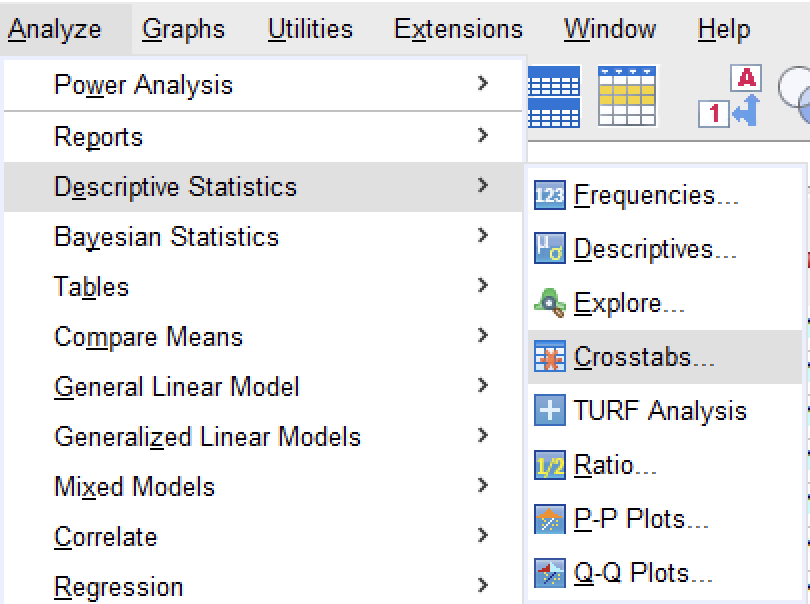
\includegraphics[width=0.49\textwidth]{figures/spss-crosstabs-menu.png}
\end{center}

در پنجره باز شده، متغیر \lr{Gender} را به قسمت \lr{Rows} و
متغیر \lr{Outcome} را به قسمت \lr{Columns} منتقل می‌کنیم. سپس روی گزینه \lr{Statistics} کلیک کرده و در پنجره باز شده، گزینه
Risk
را انتخاب می‌کنیم. سپس
Continue
و
OK
را می‌زنیم.

\begin{center}
    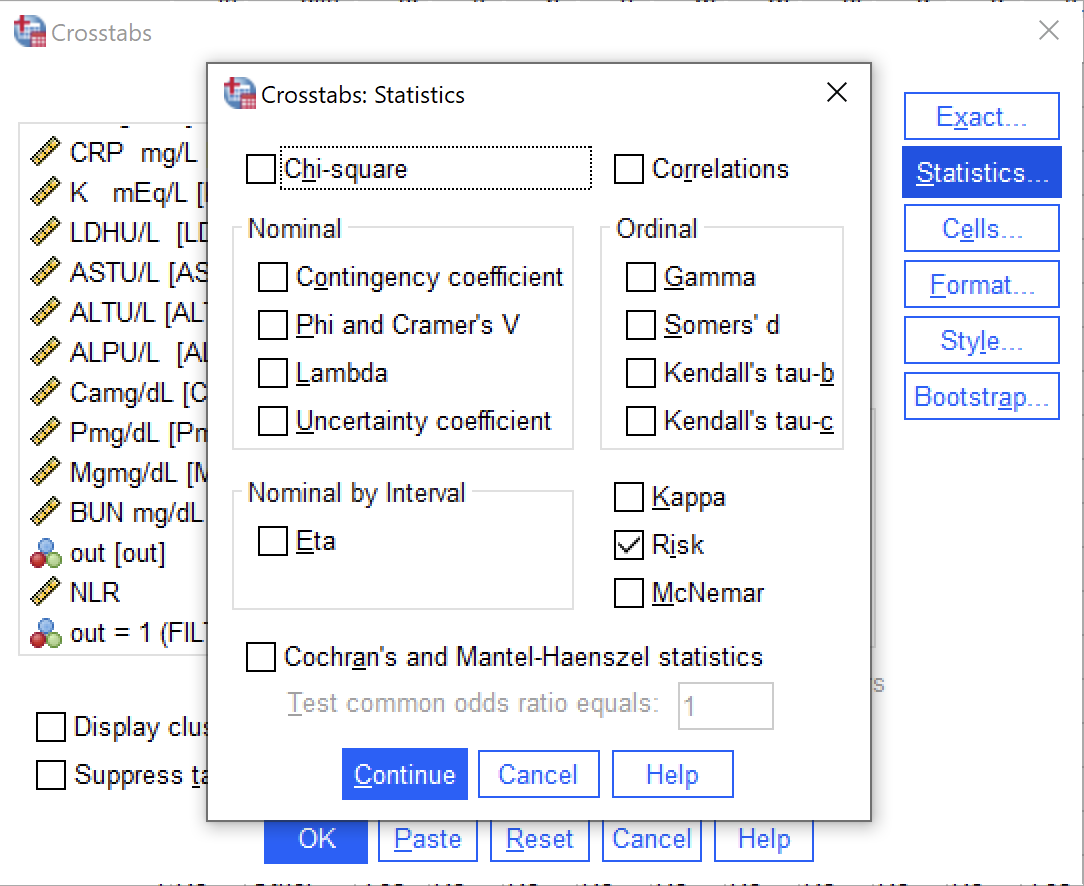
\includegraphics[width=0.45\textwidth]{figures/spss-crosstabs-statistics.png}
    \hfill
    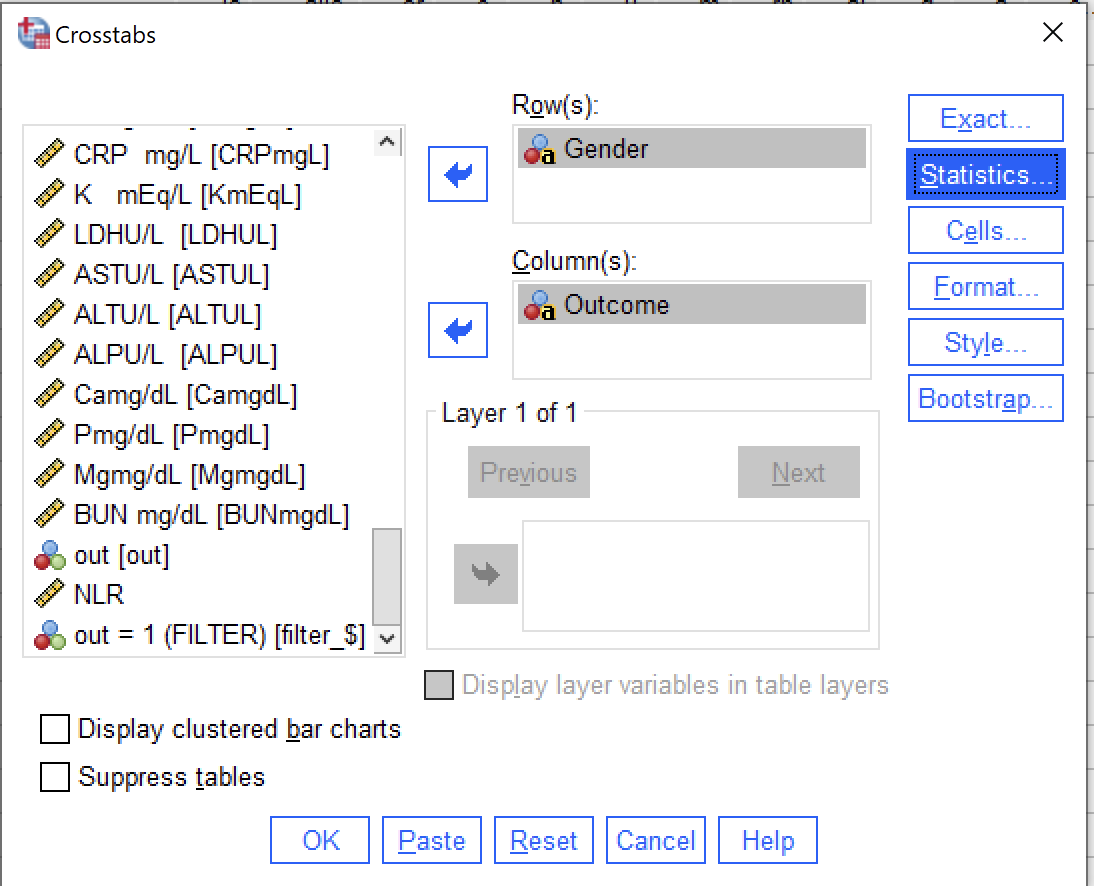
\includegraphics[width=0.45\textwidth]{figures/spss-crosstabs-dialog.png}
\end{center}

نتایج به صورت زیر نمایش داده می‌شوند:

\begin{center}
    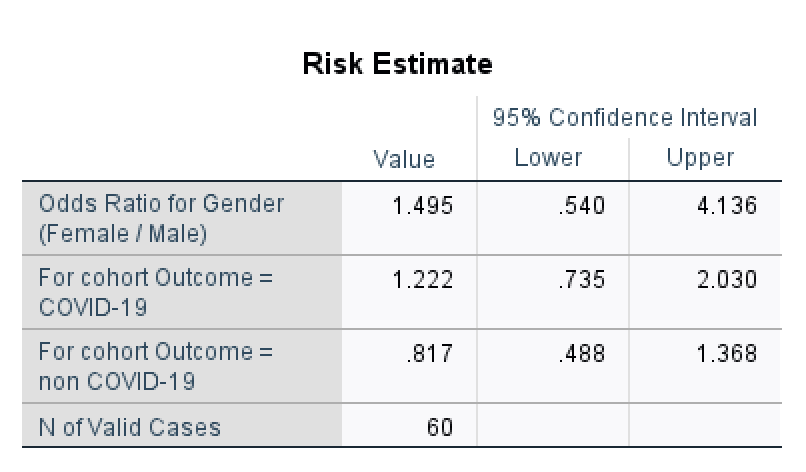
\includegraphics[width=0.45\textwidth]{figures/risk-estimate.png}
    \hfill
    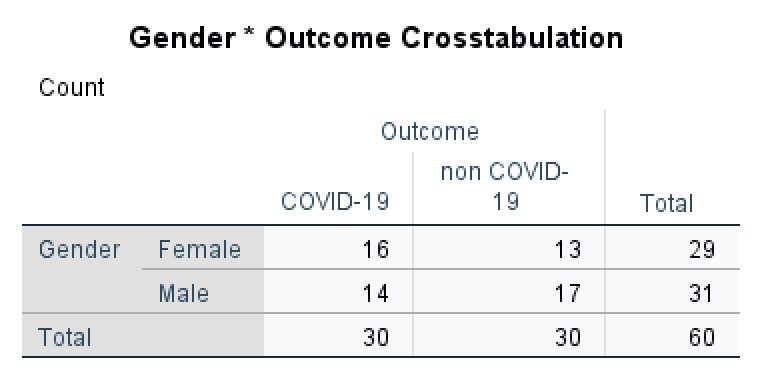
\includegraphics[width=0.45\textwidth]{figures/crosstabulation.png}
\end{center}

نتایج نشان می‌دهد که \lr{OR} برای \lr{Gender (Female / Male)} برابر با \(1.495\) است. بنابراین در این نمونه، شانس ابتلا به \lr{COVID-19} در زنان حدود \(1.495\) برابر شانس ابتلا در مردان است.
اما با توجه به اینکه بازه 
\lr{Confidence}
\(95\%\)
شامل عدد \(1\) است،
($1 \in [0.540, 4.136]$)
این نتیجه معنادار نیست و نمی‌توانیم بگوییم که جنسیت تأثیری بر بیمار بودن دارد یا خیر.

در ادامه محاسبات صورت گرفته در جدول
\lr{Risk Estimate}
را به صورت دستی نیز انجام می‌دهیم:

\begin{align*}
    \text{OR}                 & = \frac{(a/b)}{(c/d)} = \frac{a \times d}{b \times c} = \frac{16 \times 17}{13 \times 14} = \frac{136}{91} = 1.4945\ldots \approx 1.495                                      \\
    \text{SE\{ln(OR)\}}       & = \sqrt{\frac{1}{a} + \frac{1}{b} + \frac{1}{c} + \frac{1}{d}} = \sqrt{\frac{1}{16} + \frac{1}{13} + \frac{1}{14} + \frac{1}{17}} = \sqrt{\frac{6675}{24752}} \approx 0.519 \\
    \\
    \text{CI}_\text{Interval} & = exp(\ln(\text{OR}) \pm 1.96 \times \text{SE\{ln(OR)\}}) = exp(\ln(\frac{136}{91}) \pm 1.96 \times \sqrt{\frac{6675}{24752}})                                              \\
    \text{LB}                 & = exp(\ln(\text{OR}) - 1.96 \times \text{SE\{ln(OR)\}}) \approx 0.540                                                                                                       \\
    \text{UB}                 & = exp(\ln(\text{OR}) + 1.96 \times \text{SE\{ln(OR)\}}) \approx 4.136
\end{align*}

مشاهده می‌شود که نتایج کاملا منطبق با نتایج نرم‌افزار \lr{SPSS} است.
در نتیجه همانطور که اشاره شد به دلیل اینکه
$$1 \in [0.540, 4.136]$$
شواهد کافی برای نتیجه‌گیری درباره وجود ارتباط معنادار بین جنسیت و بیمار بودن وجود ندارد و
نمی‌توان جنسیت را در این تحلیل به صورت قطعی \lr{risk factor} یا \lr{protective factor} دانست.


\end{document}
